\documentclass[11pt]{article}
\usepackage[a4paper,margin=2cm]{geometry}
\usepackage[english]{babel}
\usepackage[utf8]{inputenc}
\usepackage[T1]{fontenc}
\linespread{1.3}
\parskip=12pt
\parindent=0pt
\usepackage{enumitem}
\usepackage{amsmath}
\usepackage{amsfonts}
\usepackage{graphicx}
\usepackage{amssymb}
\usepackage{hyperref}
\usepackage{amsthm}
\usepackage{color}


% Defining the question styles
\theoremstyle{definition}
\newtheorem{prob}{Problem}

% Custom commands
\newcommand{\E}{\mathbb{E}}
\newcommand{\Var}{\mathrm{Var}}
\newcommand{\Prob}{\mathbb{P}}

% declare a new theorem style
\newtheoremstyle{solution}%
{1pt}% Space above
{1pt}% Space below 
{\itshape\color{red}}% Body font
{}% Indent amount
{\bfseries\color{red}}% Theorem head font
{.}% Punctuation after theorem head
{.5em}% Space after theorem head
{}% Theorem head spec (can be left empty, meaning ‘normal’)

\theoremstyle{solution}
\newtheorem*{solution}{Solution}

% --- Code starts here ---
\begin{document}
	\begin{center}
		{\Large{\textbf{Lista IV - Métodos Numéricos}}}\\
		\vspace{0.2cm}
		EPGE - 2018\\
		Professor: Cezar Santos\\
		Aluno: Raul Guarini Riva
	\end{center}
	

O código principal da lista está no arquivo \texttt{ps4.m}. Como nas outras listas, utilizei minha função \texttt{tauchen\_ar1} para realizar a discretização desejada do processo estocástico $z_t$ num grid de 9 pontos. O problema do fazendeiro consiste em escolher consumo e número de cabras que serão guardadas em cada instante do tempo. Portanto, as variáveis de estado são o choque de dotação atual $z$ e o nível de cabras estocadas no presente $a$. As variáveis de controle são o consumo $c$ e o número de cabras a serem estocadas $a'$. A equação funcional que o fazendeiro tenta resolver, dado $q$, é dada por:
\begin{gather*}
	V(z, a) = \max\limits_{c, a'} \{ u(c) + \beta\E(V(z', a')|z)\}\\
	\text{s.t.} \quad c + qa' = e^z + a
\end{gather*}
Para a discretização do espaço de ativos, precisamos de um limite de endividamento adequado. Em geral, poderíamos utilizar o limite natural de endividamento. Contudo, neste contexto rural, parece fazer sentido definir como limite inferior para o número de cabras estocadas o valor zero. Para o limite superior, segui os slides e o defini como 40. Utilizei 2000 pontos no grid de cabras e nove pontos no grid do choque de produtividade.

Solucionei o modelo utilizando o método de iteração da função valor em vista da simplicidade de sua implementação e do quão simples é o problema do fazendeiro. A figura a seguir mostra a função valor sob a calibração original:
\begin{figure}[h!]
	\centering
	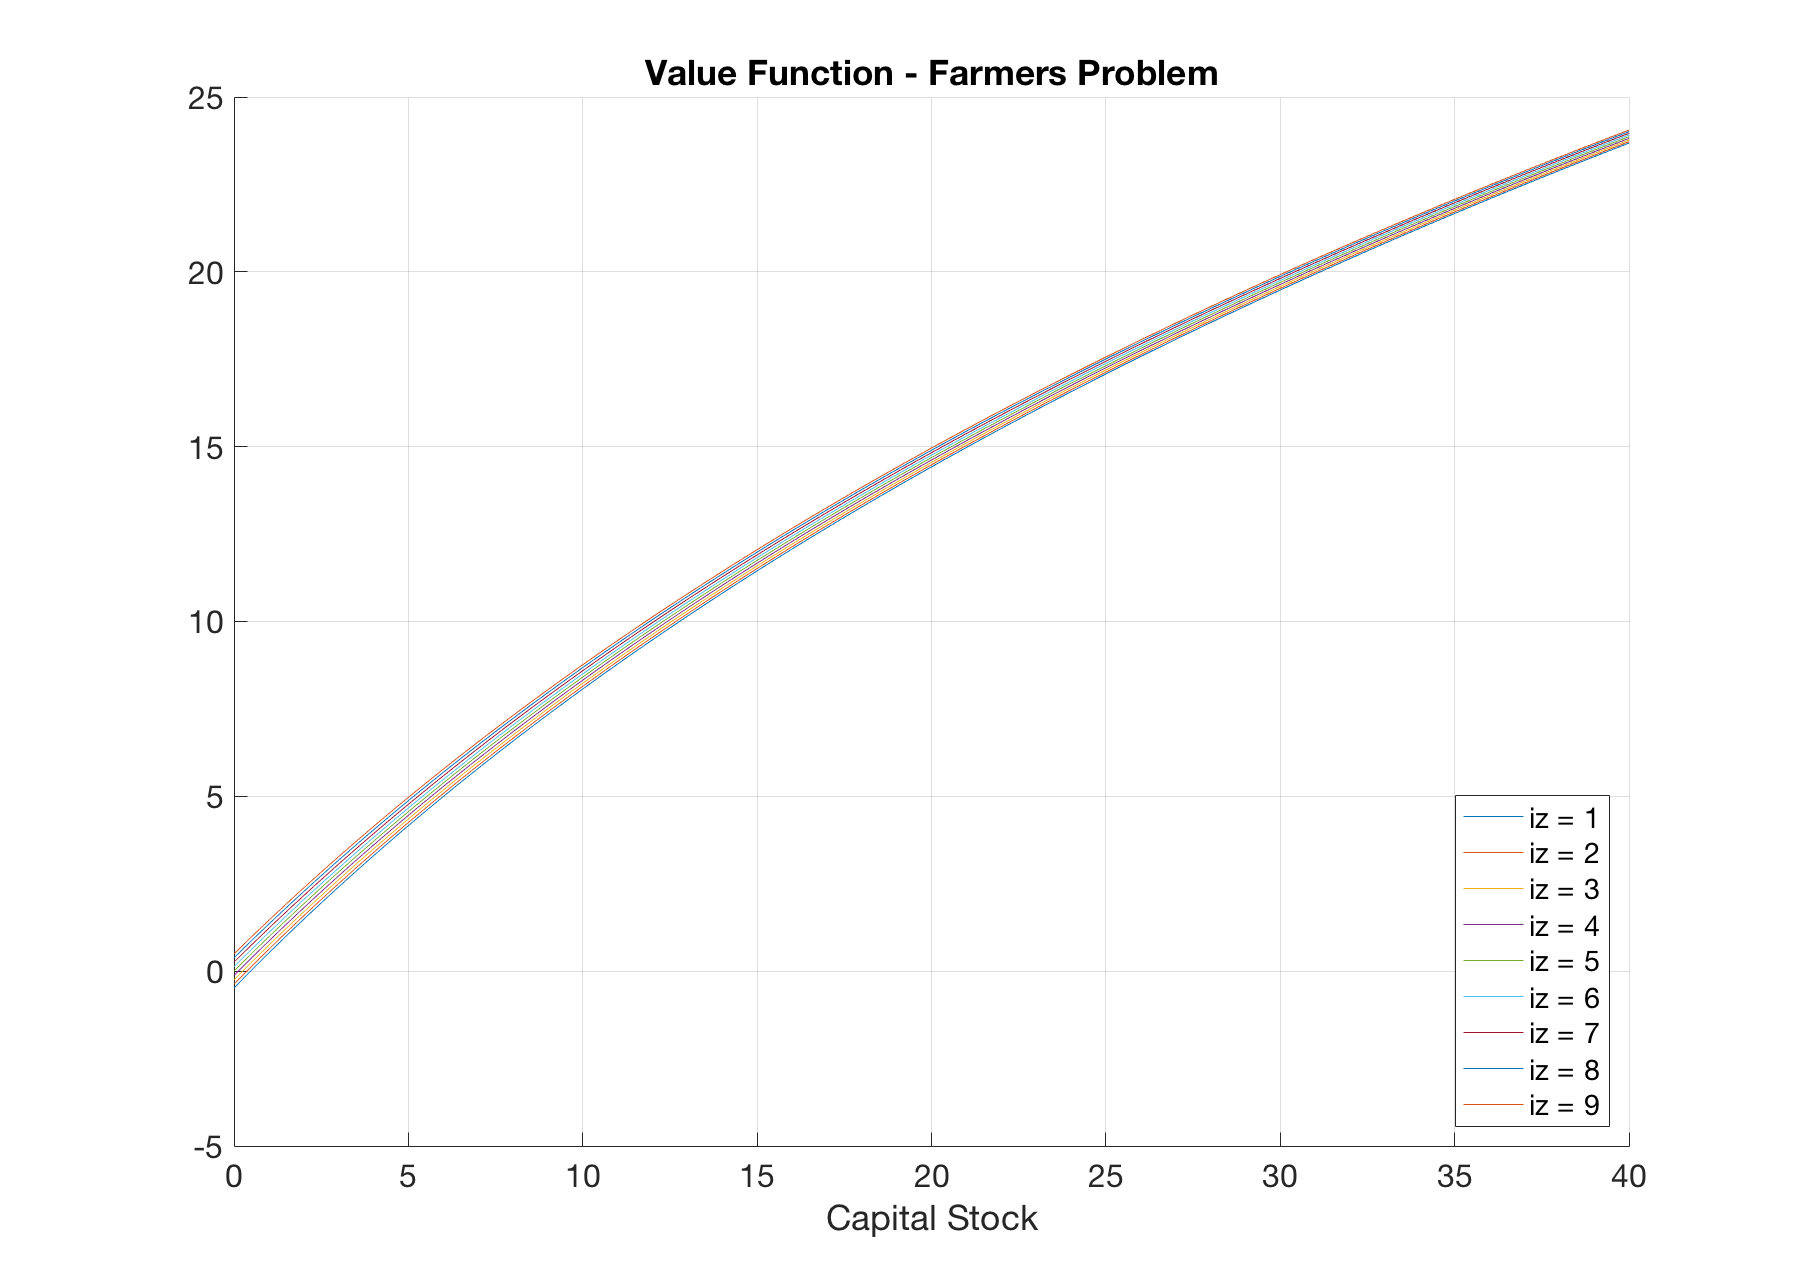
\includegraphics[scale = 0.22]{value_farmers}
\end{figure}

Em seguida, computei a distribuição estacionária, de elemento típico $\pi(z, a)$, no espaço das variáveis de estado. Utilizei o método recursivo descrito nos slides, levando em conta a cada iteração a função política de estocagem de cabras.

O código inclusive implementa um teste de robustez da solução que é checar se a soma de todas os valores da distribuição se iguala a 1.

Com base na distribuição estacionária $\pi$, computei a variável "Aggregate Goats", análoga ao que seria o capital agregado num modelo à la Hugget ou Aiyagari:
\begin{gather*}
	\text{Aggregate Goats} = \sum\limits_{a}\sum\limits_{z}g(z,a)\pi(z,a)
\end{gather*}
onde $g(z,a)$ corresponde á função política de estocagem de cabras avaliada no estado $(z,a)$, já computada no estágio anterior. A tabela abaixo mostra como esta variável se comportou em cada cenário pedido. Nos três últimos casos, apenas o parâmetro em destaque foi diferente da calibração original proposta na lista:
\begin{center}
	\begin{tabular}{c|c}
	Calibração & Aggregate Goats\\
	\hline
	\hline
	Original & 20.0093\\
	$\rho = 0.97$ & 20.0689\\
	$\gamma = 5$ & 20.0916\\
	$\sigma = 0.05$ & 20.1403
\end{tabular}
\end{center}
Com um valor maior de $\rho$, os choques tornam-se mais persistentes, ainda que o processo gerador dos choques se mantenha estacionário. Apesar da média deste processo continuar zero, um valor maior de $\rho$ implica que a variância de $z_{t}$ aumenta. Isto é, a incerteza individual com respeito à dotação de recursos aumenta. Num ambiente com mercados incompletos, os fazendeiros não podem comprar seguro contra este choque de modo que o motivo precaucional da poupança explica o maior valor agregado de cabras estocadas. Os próprios fazendeiros tentam segurar a si próprios através de poupança, evitando estados da natureza de baixo consumo, agora mais prováveis frente à maior volatilidade da dotação.

A mesma interpretação aplica-se ao caso em que $\sigma$ aumenta. Nesse caso, as inovações do processo $z_{t}$ tem maior variância, levando consequentemente à maior variância do próprio $z_{t}$. De fato, nos dois casos, o número de cabras agregadas aumenta quando comparado ao caso da calibração original.

Com $\gamma = 5$ ao invés de $\gamma = 1.0001$, os fazendeiros tornam-se mais avessos ao risco. Isto implica que oscilações no consumo causam uma desutilidade maior quando $\gamma$ cresce. A solução encontrada pelos fazendeiros para lidar com uma maior aversão ao risco é poupar mais, resultando num nível maior de cabras agregadas comparado ao caso da calibração original, algo intuitivo nesse caso.

\end{document}
